\documentclass[10pt,a4paper]{article}
\usepackage[utf8]{inputenc}
\usepackage{amsmath}
\usepackage{amsfonts}
\usepackage{amssymb}
\usepackage{graphicx}
\usepackage{epstopdf}
\usepackage[ngerman]{babel}
\usepackage[ngerman]{translator}
\usepackage[colorlinks=true,
        linkcolor=black,
        citecolor=black,
        filecolor=black,
        pagecolor=black,
        urlcolor=black,
        bookmarks=true,
        bookmarksopen=true,
        bookmarksopenlevel=3,
        plainpages=false,
        pdfpagelabels=true]{hyperref}

\parindent 0pt
\pagestyle{headings}

\let\oldsection\section
\renewcommand{\section}{\newpage \oldsection}

\title{
	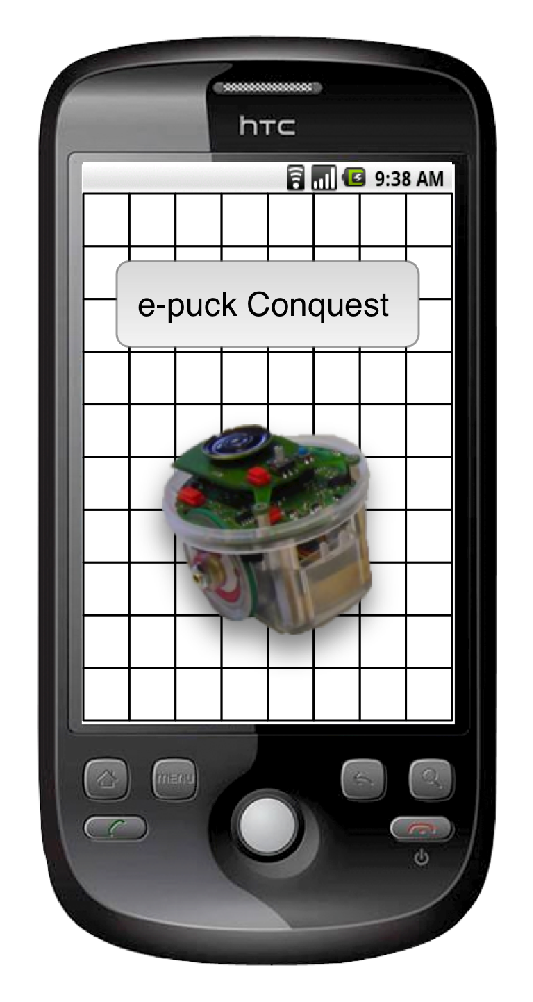
\includegraphics[height=10cm]{logo.eps} \\
	\vspace{1cm}
	Entwurf
}
\author{Lorenz Flo} 
\begin{document}

% Das ist der Titel
	Die Proxy-Klasse implementiert \textit{IRobot} und besteht aus einem Thread, der für die Verarbeitungslogik von
	Informationen zuständig ist. Diese Klasse repräsentiert die Schnittstelle zwischen einem e-puck Roboter und der
	\textit{Environment}-Klasse. \\
	Hauptaufgaben, welche größtenteils vom \textit{LogicThread} wahrgenommen werden:
	\begin{itemize}
		\item Nachrichtenaustausch mit dem e-puck \\
			Über den Bluetooth-Socket werden Daten vom e-puck Roboter empfangen und gesendet.
		\item Senden von Broadcast-Nachrichten \\
			Mit Hilfe der \textit{broadcast()}-Methode der \textit{Environment}-Klasse können Nachrichten an alle
			e-puck Proxies sowie an das \textit{Environment} selbst, übermittelt werden. \\
			Diese Nachrichten enthalten	Zustandsupdates, die für alle Teilnehmer relevant sind. Darunter fallen z.B.
			Positionsupdates, Kartenupdates oder Nachrichten der abstrakten Logik.
		\item Empfangen von Nachrichten  \\
			Nachricht werden über die \textit{deliver()}-Methode angenommen und durch das Chain-of-Responsibility
			-Pattern verarbeitet.
		\item Zustandsbeschreibung aller e-puck Roboter \\
			Mithilfe von \textit{Positioning}-Objekten wird der aktuelle Zustand aller e-puck Roboter lokal gespeichert.
		\item Verwaltung der lokalen Karte \\
			Die lokale \textit{GridMap} muss sowohl bei lokalen als auch bei entfernten Updates aktualisiert werden. 
		\item Umsetzung von Benutzereingaben \\
			Geschwindigkeitsänderungen sowie Fahrtanweisungen durch den Benutzer werden verarbeitet und gegebenenfalls
			an den e-puck weitergeleitet.
		\item Management der künstlichen Intelligenz \\
			Hierunter fällt die Anwendung der abstrakten Logik wie z.B. Erkundung und Kollisionsvermeidung.
	\end{itemize}
	

						
\end{document}